%%%%%%%%%%%%%%%%%%%%%%%%%%%%%%%%%%%%%%%%%
% Beamer Presentation
% LaTeX Template
% Version 2.0 (March 8, 2022)
%
% This template originates from:
% https://www.LaTeXTemplates.com
%
% Author:
% Vel (vel@latextemplates.com)
%
% License:
% CC BY-NC-SA 4.0 (https://creativecommons.org/licenses/by-nc-sa/4.0/)
%
%%%%%%%%%%%%%%%%%%%%%%%%%%%%%%%%%%%%%%%%%

%----------------------------------------------------------------------------------------
%	PACKAGES AND OTHER DOCUMENT CONFIGURATIONS
%----------------------------------------------------------------------------------------
\documentclass[
  24pt, % Set the default font size, options include: 8pt, 9pt, 10pt, 11pt, 12pt, 14pt, 17pt, 20pt
  %t, % Uncomment to vertically align all slide content to the top of the slide, rather than the default centered
  aspectratio=169, % Uncomment to set the aspect ratio to a 16:9 ratio which matches the aspect ratio of 1080p and 4K screens and projectors
]{beamer}

\graphicspath{{Images/}{./}} % Specifies where to look for included images (trailing slash required)

\usepackage{booktabs} % Allows the use of \toprule, \midrule and \bottomrule for better rules in tables

%----------------------------------------------------------------------------------------
%	SELECT LAYOUT THEME
%----------------------------------------------------------------------------------------

% Beamer comes with a number of default layout themes which change the colors and layouts of slides. Below is a list of all themes available, uncomment each in turn to see what they look like.

%\usetheme{default}
%\usetheme{AnnArbor}
%\usetheme{Antibes}
%\usetheme{Bergen}
%\usetheme{Berkeley}
%\usetheme{Berlin}
\usetheme{Boadilla} %me gusta
%\usetheme{CambridgeUS}
%\usetheme{Copenhagen}
%\usetheme{Darmstadt}
%\usetheme{Dresden}
%\usetheme{Frankfurt}
%\usetheme{Goettingen} %dos dos
%\usetheme{Hannover} %dos dos
%\usetheme{Ilmenau}
%\usetheme{JuanLesPins}
%\usetheme{Luebeck}
%\usetheme{Madrid}
%\usetheme{Malmoe}
%\usetheme{Marburg}
%\usetheme{Montpellier}
%\usetheme{PaloAlto}
%\usetheme{Pittsburgh}
%\usetheme{Rochester} %muy flat
%\usetheme{Singapore}
%\usetheme{Szeged}
%\usetheme{Warsaw}

%----------------------------------------------------------------------------------------
%	SELECT COLOR THEME
%----------------------------------------------------------------------------------------

% Beamer comes with a number of color themes that can be applied to any layout theme to change its colors. Uncomment each of these in turn to see how they change the colors of your selected layout theme.

%\usecolortheme{albatross}
%\usecolortheme{beaver}
%\usecolortheme{beetle}
%\usecolortheme{crane}
%\usecolortheme{dolphin}
%\usecolortheme{dove}
%\usecolortheme{fly}
%\usecolortheme{lily} %default
%\usecolortheme{monarca}
%\usecolortheme{seagull}
%\usecolortheme{seahorse}
%\usecolortheme{spruce}
%\usecolortheme{whale}
%\usecolortheme{wolverine}

%----------------------------------------------------------------------------------------
%	SELECT FONT THEME & FONTS
%----------------------------------------------------------------------------------------

% Beamer comes with several font themes to easily change the fonts used in various parts of the presentation. Review the comments beside each one to decide if you would like to use it. Note that additional options can be specified for several of these font themes, consult the beamer documentation for more information.

\usefonttheme{default} % Typeset using the default sans serif font
%\usefonttheme{serif} % Typeset using the default serif font (make sure a sans font isn't being set as the default font if you use this option!)
%\usefonttheme{structurebold} % Typeset important structure text (titles, headlines, footlines, sidebar, etc) in bold
%\usefonttheme{structureitalicserif} % Typeset important structure text (titles, headlines, footlines, sidebar, etc) in italic serif
%\usefonttheme{structuresmallcapsserif} % Typeset important structure text (titles, headlines, footlines, sidebar, etc) in small caps serif

%------------------------------------------------

%\usepackage{mathptmx} % Use the Times font for serif text
\usepackage{palatino} % Use the Palatino font for serif text

\usepackage[ruled,vlined]{algorithm2e}
%\usepackage{helvet} % Use the Helvetica font for sans serif text
\usepackage[default]{opensans} % Use the Open Sans font for sans serif text
\usepackage[spanish]{babel}
\usepackage{dirtree}
\usepackage{xcolor}
%\usepackage[default]{FiraSans} % Use the Fira Sans font for sans serif text
%\usepackage[default]{lato} % Use the Lato font for sans serif text

\usepackage[scaled]{helvet}
\usepackage[round]{natbib}
%\newcommand{\newblock}{}

\usepackage{rotating}

\newcommand\FourQuad[4]{%
  \begin{minipage}[b][.33\textheight][t] 
    {.48\textwidth}#1\end{minipage}\hfill%
    \begin{minipage}[b][.33\textheight][t] 
      {.48\textwidth}#2\end{minipage}\\[0.5em]
      \begin{minipage}[b][.33\textheight][t] 
        {.48\textwidth}#3\end{minipage}\hfill
        \begin{minipage}[b][.33\textheight][t] 
          {.48\textwidth}#4\end{minipage}%
}

\usepackage{tikz}
%\usetikzlibrary{arrows,shapes,positioning,shadows,trees,quotes}


%\tikzset{
%  basic/.style  = {draw, text width=2cm, drop shadow, font=\sffamily, rectangle},
%  root/.style   = {basic, rounded corners=2pt, thin, align=center,
%                   fill=green!30},
%  level 2/.style = {basic, rounded corners=6pt, thin,align=center, fill=green!60,
%                   text width=8em},
%  level 3/.style = {basic, thin, align=left, fill=pink!60, text width=6.5em}
%}

\usetikzlibrary{calc}

\tikzstyle{part} = [rectangle, rounded corners, minimum width=3cm, minimum height=1cm,     align=center, draw=black]
\tikzstyle{chapter} = [rectangle, rounded corners, minimum width=3cm, minimum height=1cm,     align=center, draw=black, text width=3.5cm]
\tikzstyle{arrow} = [thick, ->]

\usepackage{array} % needed for \arraybackslash
\usepackage{graphicx}
\usepackage{adjustbox} % for \adjincludegraphics

\usepackage{subcaption}
\usepackage{bibentry}
%\bibliographystyle{apalike}
\usepackage{chngcntr}
\usepackage{lipsum}% http://ctan.org/pkg/lipsum
\usepackage{hanging}% http://ctan.org/pkg/hanging

\usepackage{xcolor,colortbl}
\usepackage{multirow}

\usepackage{animate}
\usepackage{multicol}
\usepackage{tabularx,booktabs}
\usepackage{forloop}
\usepackage{ragged2e}

\usepackage{bbding} %palomitas checkmark
\usepackage{pifont}

\newcounter{loopcntr}
%----------------------------------------------------------------------------------------
%	SELECT INNER THEME
%----------------------------------------------------------------------------------------

% Inner themes change the styling of internal slide elements, for example: bullet points, blocks, bibliography entries, title pages, theorems, etc. Uncomment each theme in turn to see what changes it makes to your presentation.

%\useinnertheme{default}
\useinnertheme{circles}
%\useinnertheme{rectangles}
%\useinnertheme{rounded}
%\useinnertheme{inmargin}

%----------------------------------------------------------------------------------------
%	SELECT OUTER THEME
%----------------------------------------------------------------------------------------

% Outer themes change the overall layout of slides, such as: header and footer lines, sidebars and slide titles. Uncomment each theme in turn to see what changes it makes to your presentation.

%\useoutertheme{default}
%\useoutertheme{infolines}
%\useoutertheme{miniframes}
%\useoutertheme{smoothbars}
%\useoutertheme{sidebar}
%\useoutertheme{split}
%\useoutertheme{shadow}
%\useoutertheme{tree}
%\useoutertheme{smoothtree}

%\setbeamertemplate{footline} % Uncomment this line to remove the footer line in all slides
\setbeamertemplate{footline}[page number] % Uncomment this line to replace the footer line in all slides with a simple slide count
%\setbeamertemplate{caption}[numbered]
\setbeamertemplate{navigation symbols}{} % Uncomment this line to remove the navigation symbols from the bottom of all slides

%----------------------------------------------------------------------------------------
%	PRESENTATION INFORMATION
%----------------------------------------------------------------------------------------

\title[PROTOCOLO DE INVESTIGACIÓN]{%\centering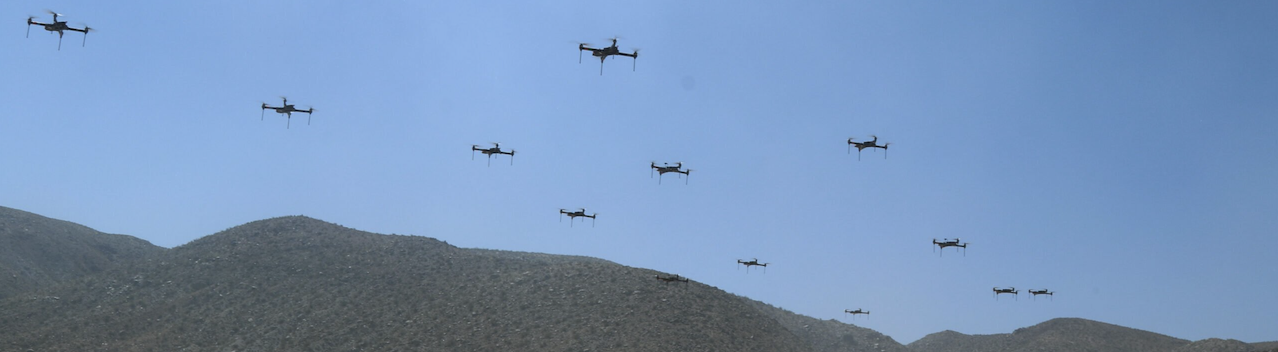
\includegraphics[width=10cm]{swarm_drones}\\
  Estrategias para la exploración coordinada multi-VANT} % The short title in the optional parameter appears at the bottom of every slide, the full title in the main parameter is only on the title page

%\subtitle{Optional Subtitle} % Presentation subtitle, remove this command if a subtitle isn't required

\author[Luis Ballado]{Luis Alberto Ballado Aradias} % Presenter name(s), the optional parameter can contain a shortened version to appear on the bottom of every slide, while the main parameter will appear on the title slide

\institute[CINVESTAV]{
  CINVESTAV UNIDAD TAMAULIPAS \\
  %\smallskip \textit{luis.ballado@cinvestav.mx}
} % Your institution, the optional parameter can be used for the institution shorthand and will appear on the bottom of every slide after author names, while the required parameter is used on the title slide and can include your email address or additional information on separate lines

\date[\today]{Cd. Victoria, Tamaulipas - \today} % Presentation date or conference/meeting name, the optional parameter can contain a shortened version to appear on the bottom of every slide, while the required parameter value is output to the title slide

%\titlegraphic{\hspace*{8.75cm}~%
%   
\includegraphics[width=0.8cm]{cinvestavlogo}
%}

%----------------------------------------------------------------------------------------

\counterwithin*{footnote}{page}
\newcommand\footcite[1]{\footnote{\bibentry{#1}}\label{\thepage:#1}}
\newcommand\secondcite[1]{\textsuperscript{\ref{\thepage:#1}}}

\newcommand{\rpt}[2][1]{%
  \forloop{loopcntr}{0}{\value{loopcntr}<#1}{#2}%
}
\newcommand{\on}[1][1]{
  \forloop{loopcntr}{0}{\value{loopcntr}<#1}{&\cellcolor{gray}}
}
\newcommand{\off}[1][1]{
  \forloop{loopcntr}{0}{\value{loopcntr}<#1}{&}
}

\addtolength{\textheight}{90pt}

\newcommand{\I}{\mathbb{I}}
\newcommand{\K}{\mathbb{K}}
\newcommand{\N}{\mathbb{N}}
\newcommand{\Q}{\mathbb{Q}}
\newcommand{\R}{\mathbb{R}}
\newcommand{\Z}{\mathbb{Z}}

\newcommand{\specialcell}[2][c]{%
  \begin{tabular}[#1]{@{}c@{}}#2\end{tabular}}


\begin{document}

%----------------------------------------------------------------------------------------
%	TITLE SLIDE
%----------------------------------------------------------------------------------------

\begin{frame}
  \titlepage % Output the title slide, automatically created using the text entered in the PRESENTATION INFORMATION block above
\end{frame}

%----------------------------------------------------------------------------------------
%	TABLE OF CONTENTS SLIDE
%----------------------------------------------------------------------------------------

% The table of contents outputs the sections and subsections that appear in your presentation, specified with the standard \section and \subsection commands. You may either display all sections and subsections on one slide with \tableofcontents, or display each section at a time on subsequent slides with \tableofcontents[pausesections]. The latter is useful if you want to step through each section and mention what you will discuss.
\AtBeginSection[]
{
  \begin{frame}
    \frametitle{Contenido} % Slide title, remove this command for no title
    \tableofcontents[currentsection] % Output the table of contents (all sections on one slide)
    %\tableofcontents[pausesections] % Output the table of contents (break sections up across separate slides)
  \end{frame}
}
%----------------------------------------------------------------------------------------
%	PRESENTATION BODY SLIDES
%----------------------------------------------------------------------------------------

\section{Resumen}
\begin{frame}{Resumen}%{Problemática}
  \bigskip % Vertical whitespace
  \centering
  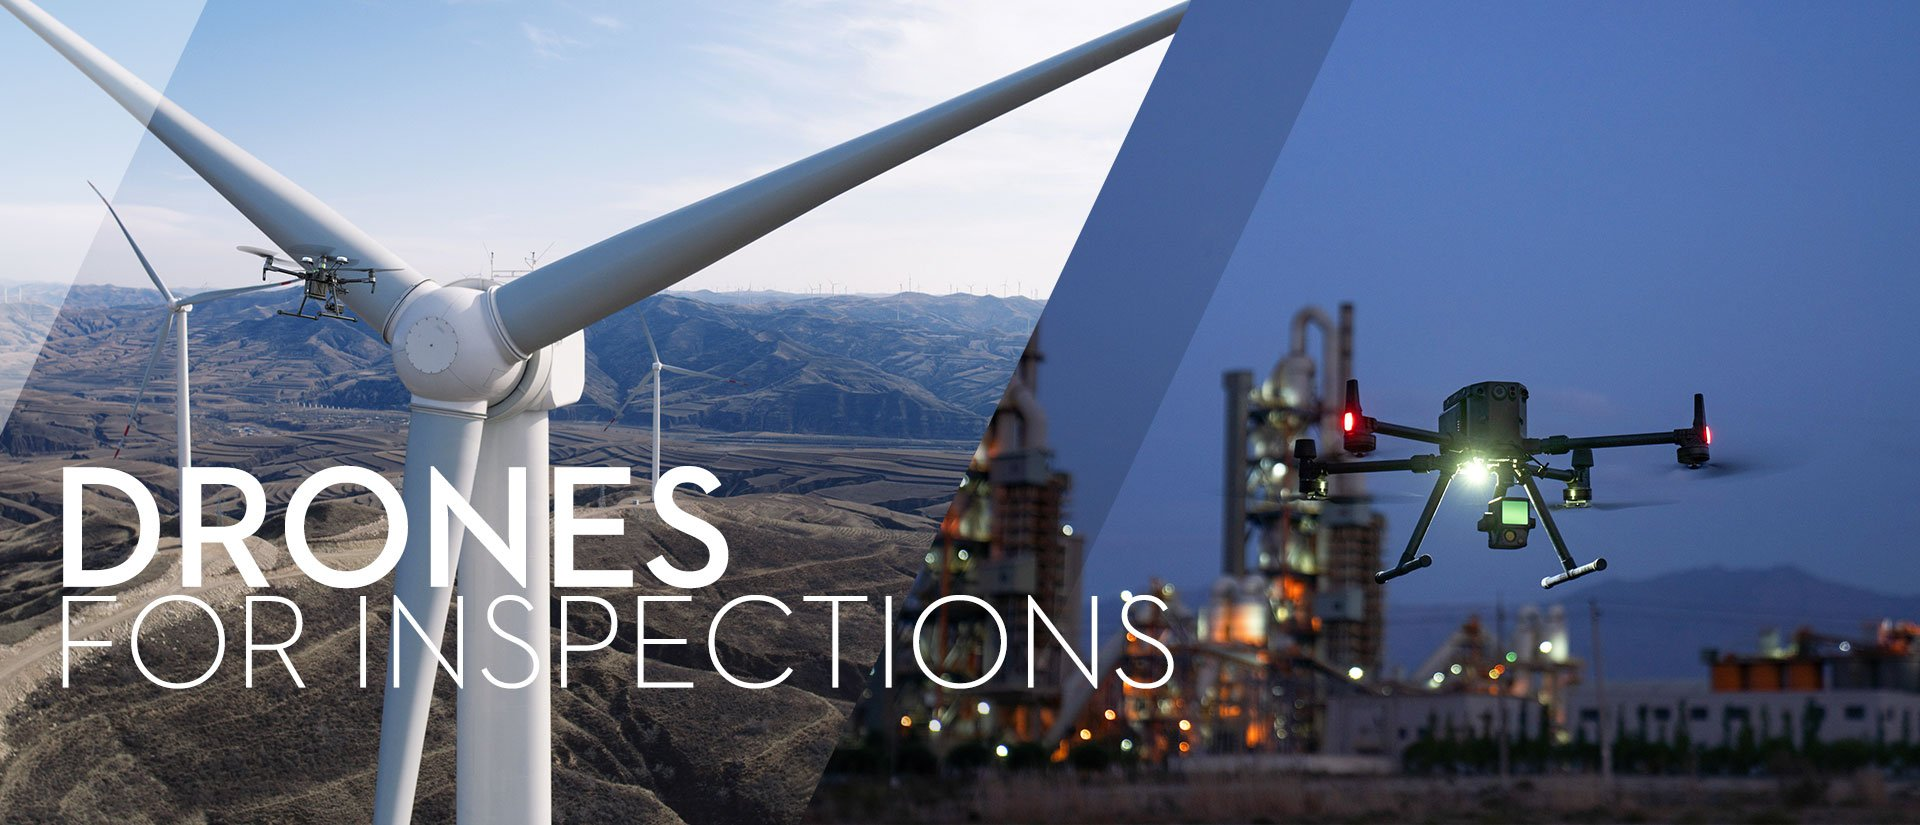
\includegraphics[width=0.45\textwidth,height=0.35\textheight]{DJI_B1}$^\dag$
  \hfil
  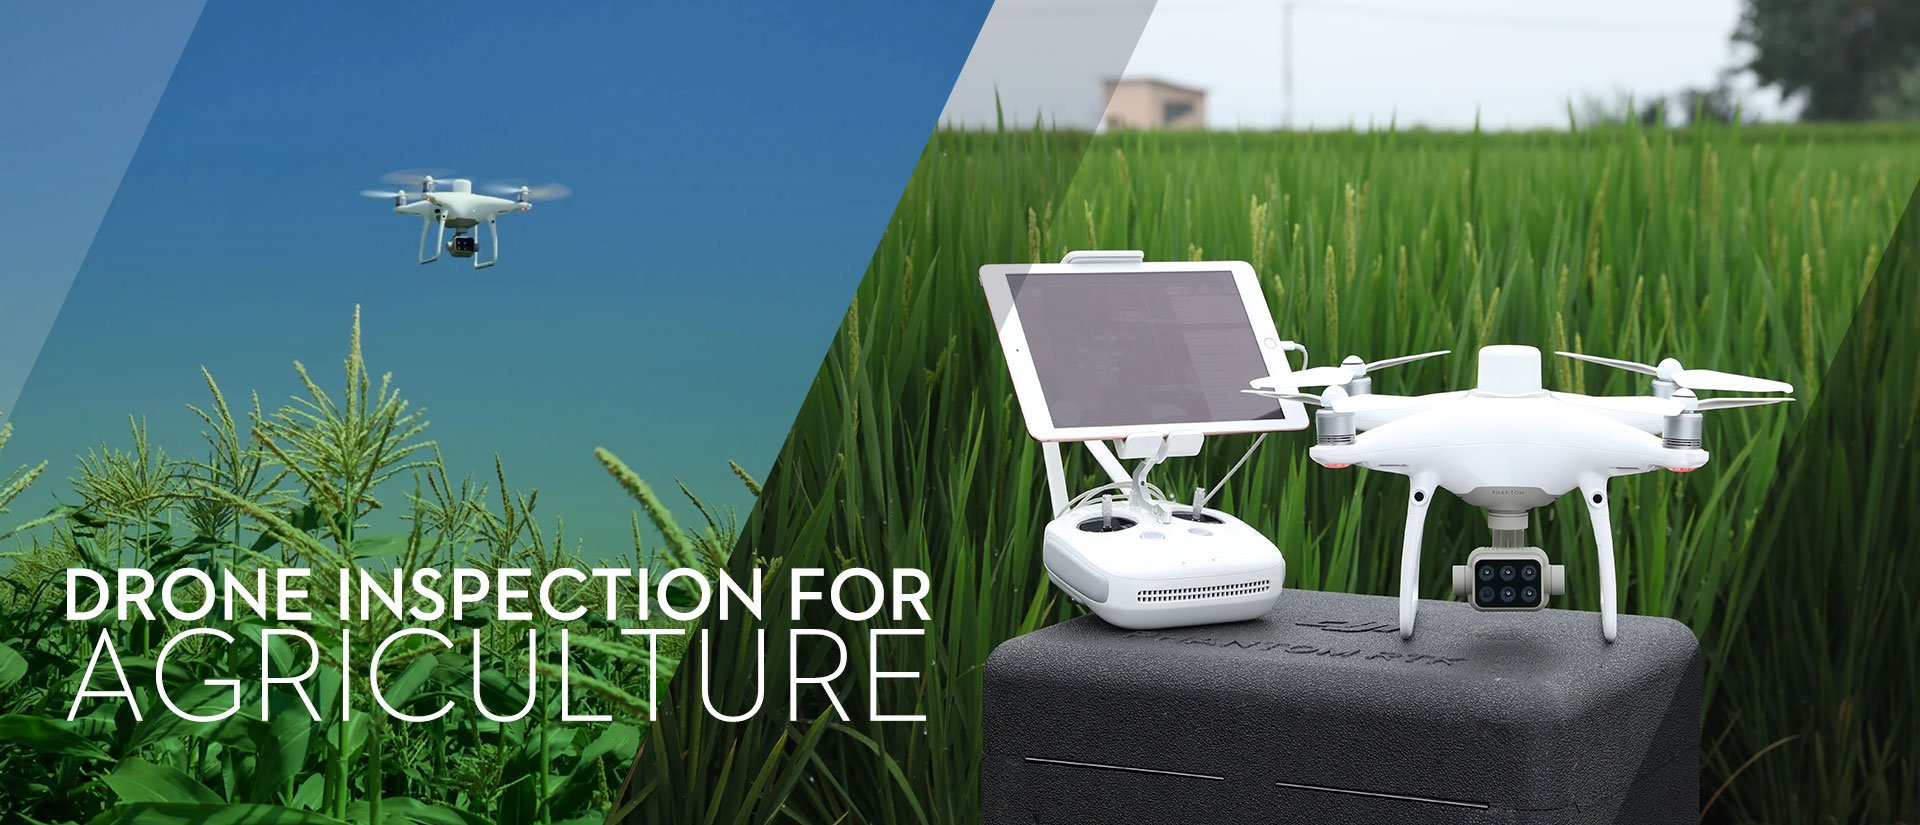
\includegraphics[width=0.45\textwidth,height=0.35\textheight]{DJI_B2}$^\dag$
  \vspace{2pt}
  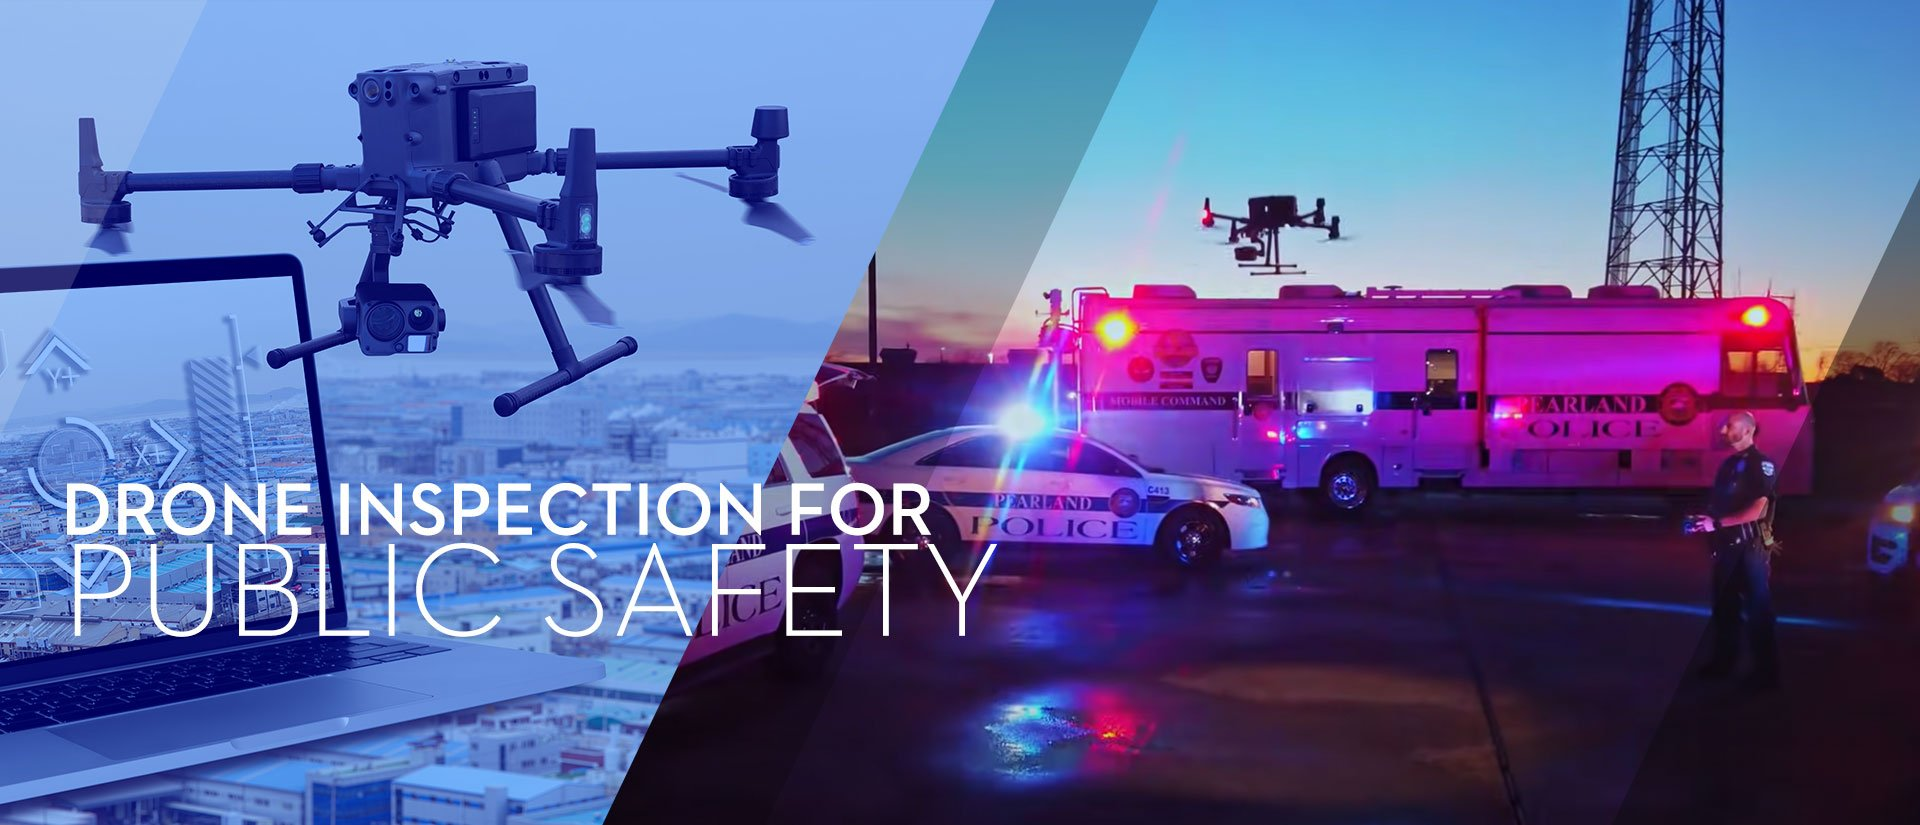
\includegraphics[width=0.45\textwidth,height=0.35\textheight]{DJI_B5}$^\dag$ 
  \hfil
  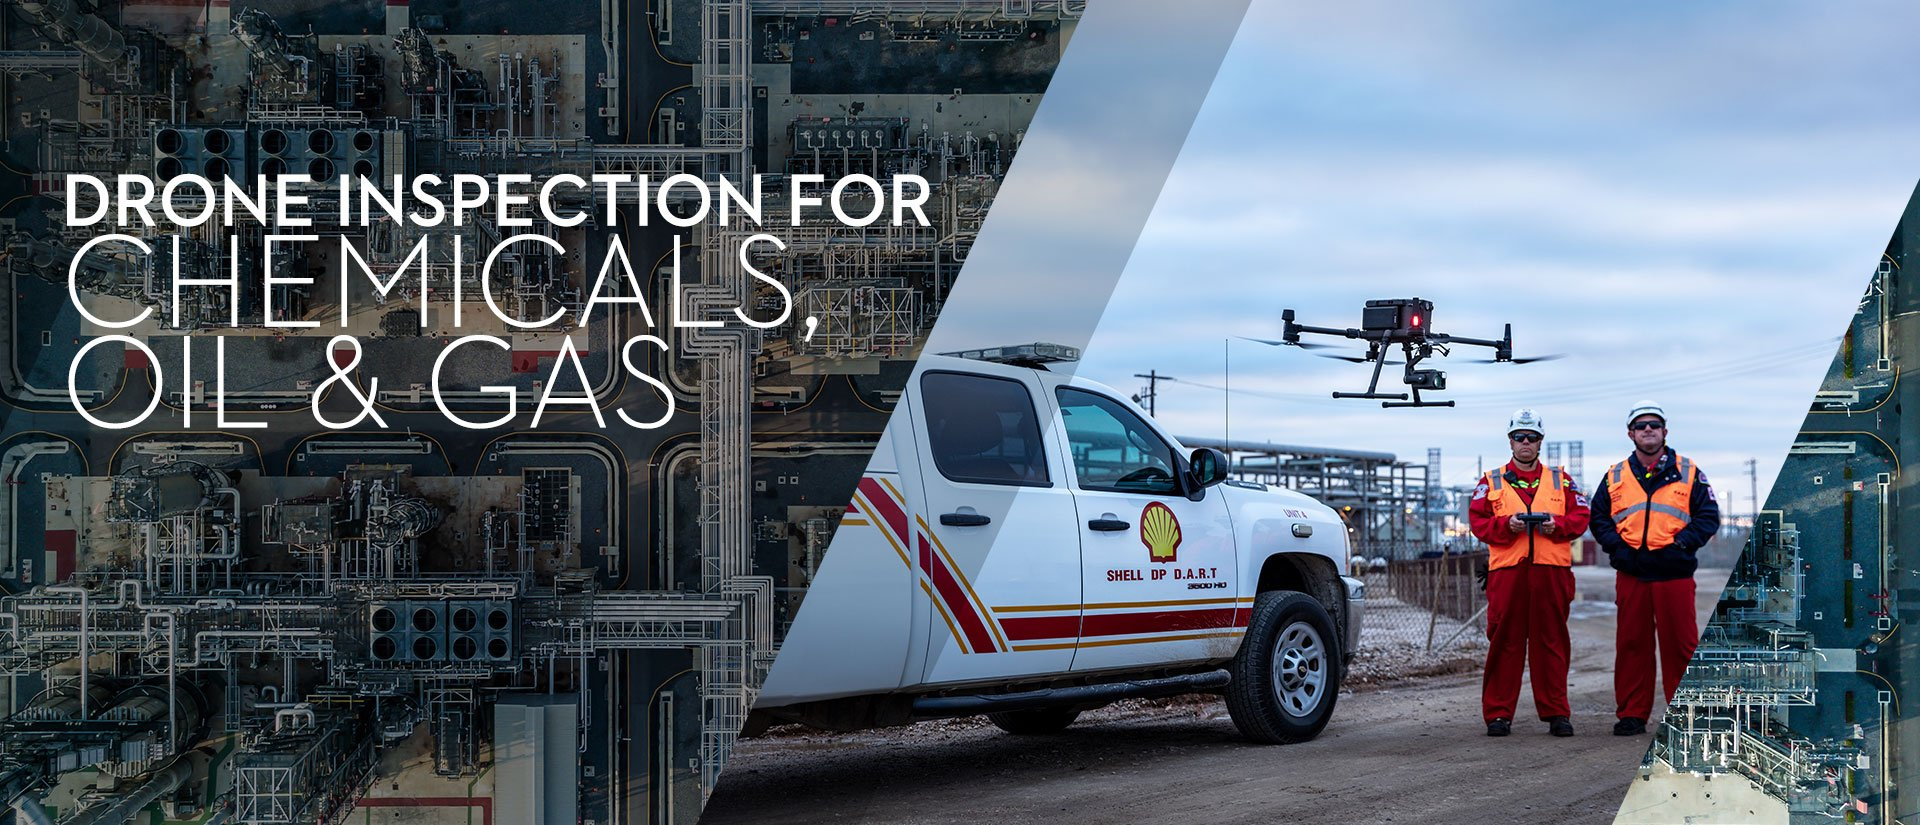
\includegraphics[width=0.45\textwidth,height=0.35\textheight]{DJI_B4}$^\dag$\\
  \rule{0in}{1.2em}$^\dag$ \small Inspecciones con VANT basadas en los mejores casos de uso\\
  \tiny \url{https://enterprise-insights.dji.com/blog/complete-guide-to-drone-inspections}
\end{frame}

\section{Descripción del proyecto}
\begin{frame}{Descripción del proyecto}
  \begin{minipage}{0.47\textwidth}
    \begin{itemize}
    \item<1-> Coordinación para la exploración multi-VANT 
    \item<2-> Optimización de rutas multi-VANT % la cobertura en entornos complejos
    \item<3-> Toma de decisiones colaborativa
    \item<4-> Evasión de obstáculos y coordinación en tiempo real
    \item<5-> Fusión de información (sensores y navegación)
    \end{itemize}
  \end{minipage}
  \begin{minipage}{0.5\textwidth}
    \only<1>{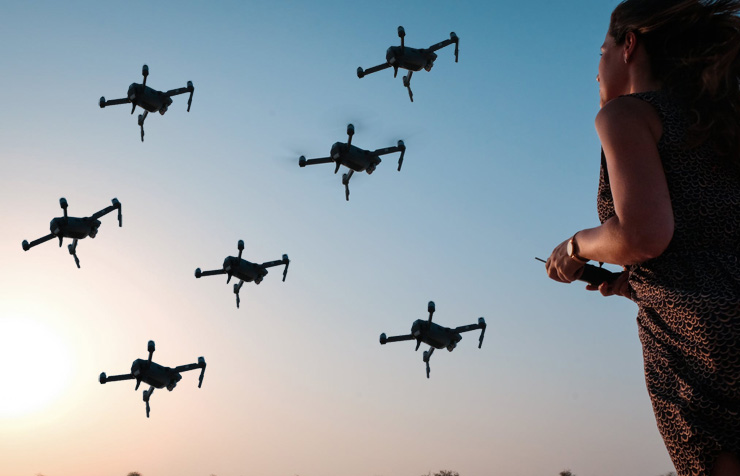
\includegraphics[width=\textwidth]{multiple-drones}$^\dag$\\
      \rule{0in}{1.2em}$^\dag$\scriptsize Ilustración Multi-VAN \\
      \tiny \url{https://dronevideos.com/} 
    }
    \only<2>{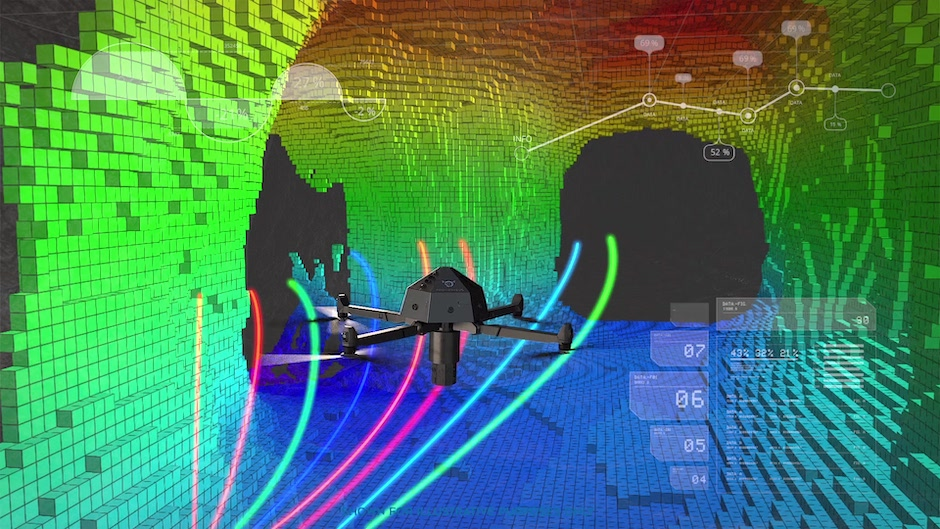
\includegraphics[width=\textwidth]{drone_path}$^\dag$\\
      \rule{0in}{1.2em}$^\dag$\scriptsize Exploración VANT en entorno 3D. \\
      \url{https://www.theengineer.co.uk/content/news/prometheus-drones-to-explore-subterranean-environments/} 
    }
    \only<3>{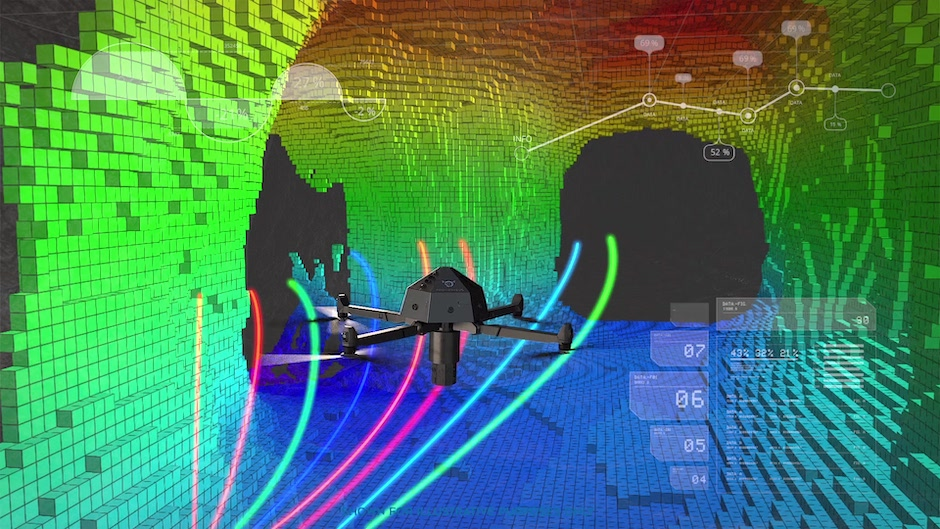
\includegraphics[width=\textwidth]{drone_path}$^\dag$\\
      \rule{0in}{1.2em}$^\dag$\scriptsize Exploración VANT en entorno 3D. \\
      \url{https://www.theengineer.co.uk/content/news/prometheus-drones-to-explore-subterranean-environments/} 
    }
    \only<4>{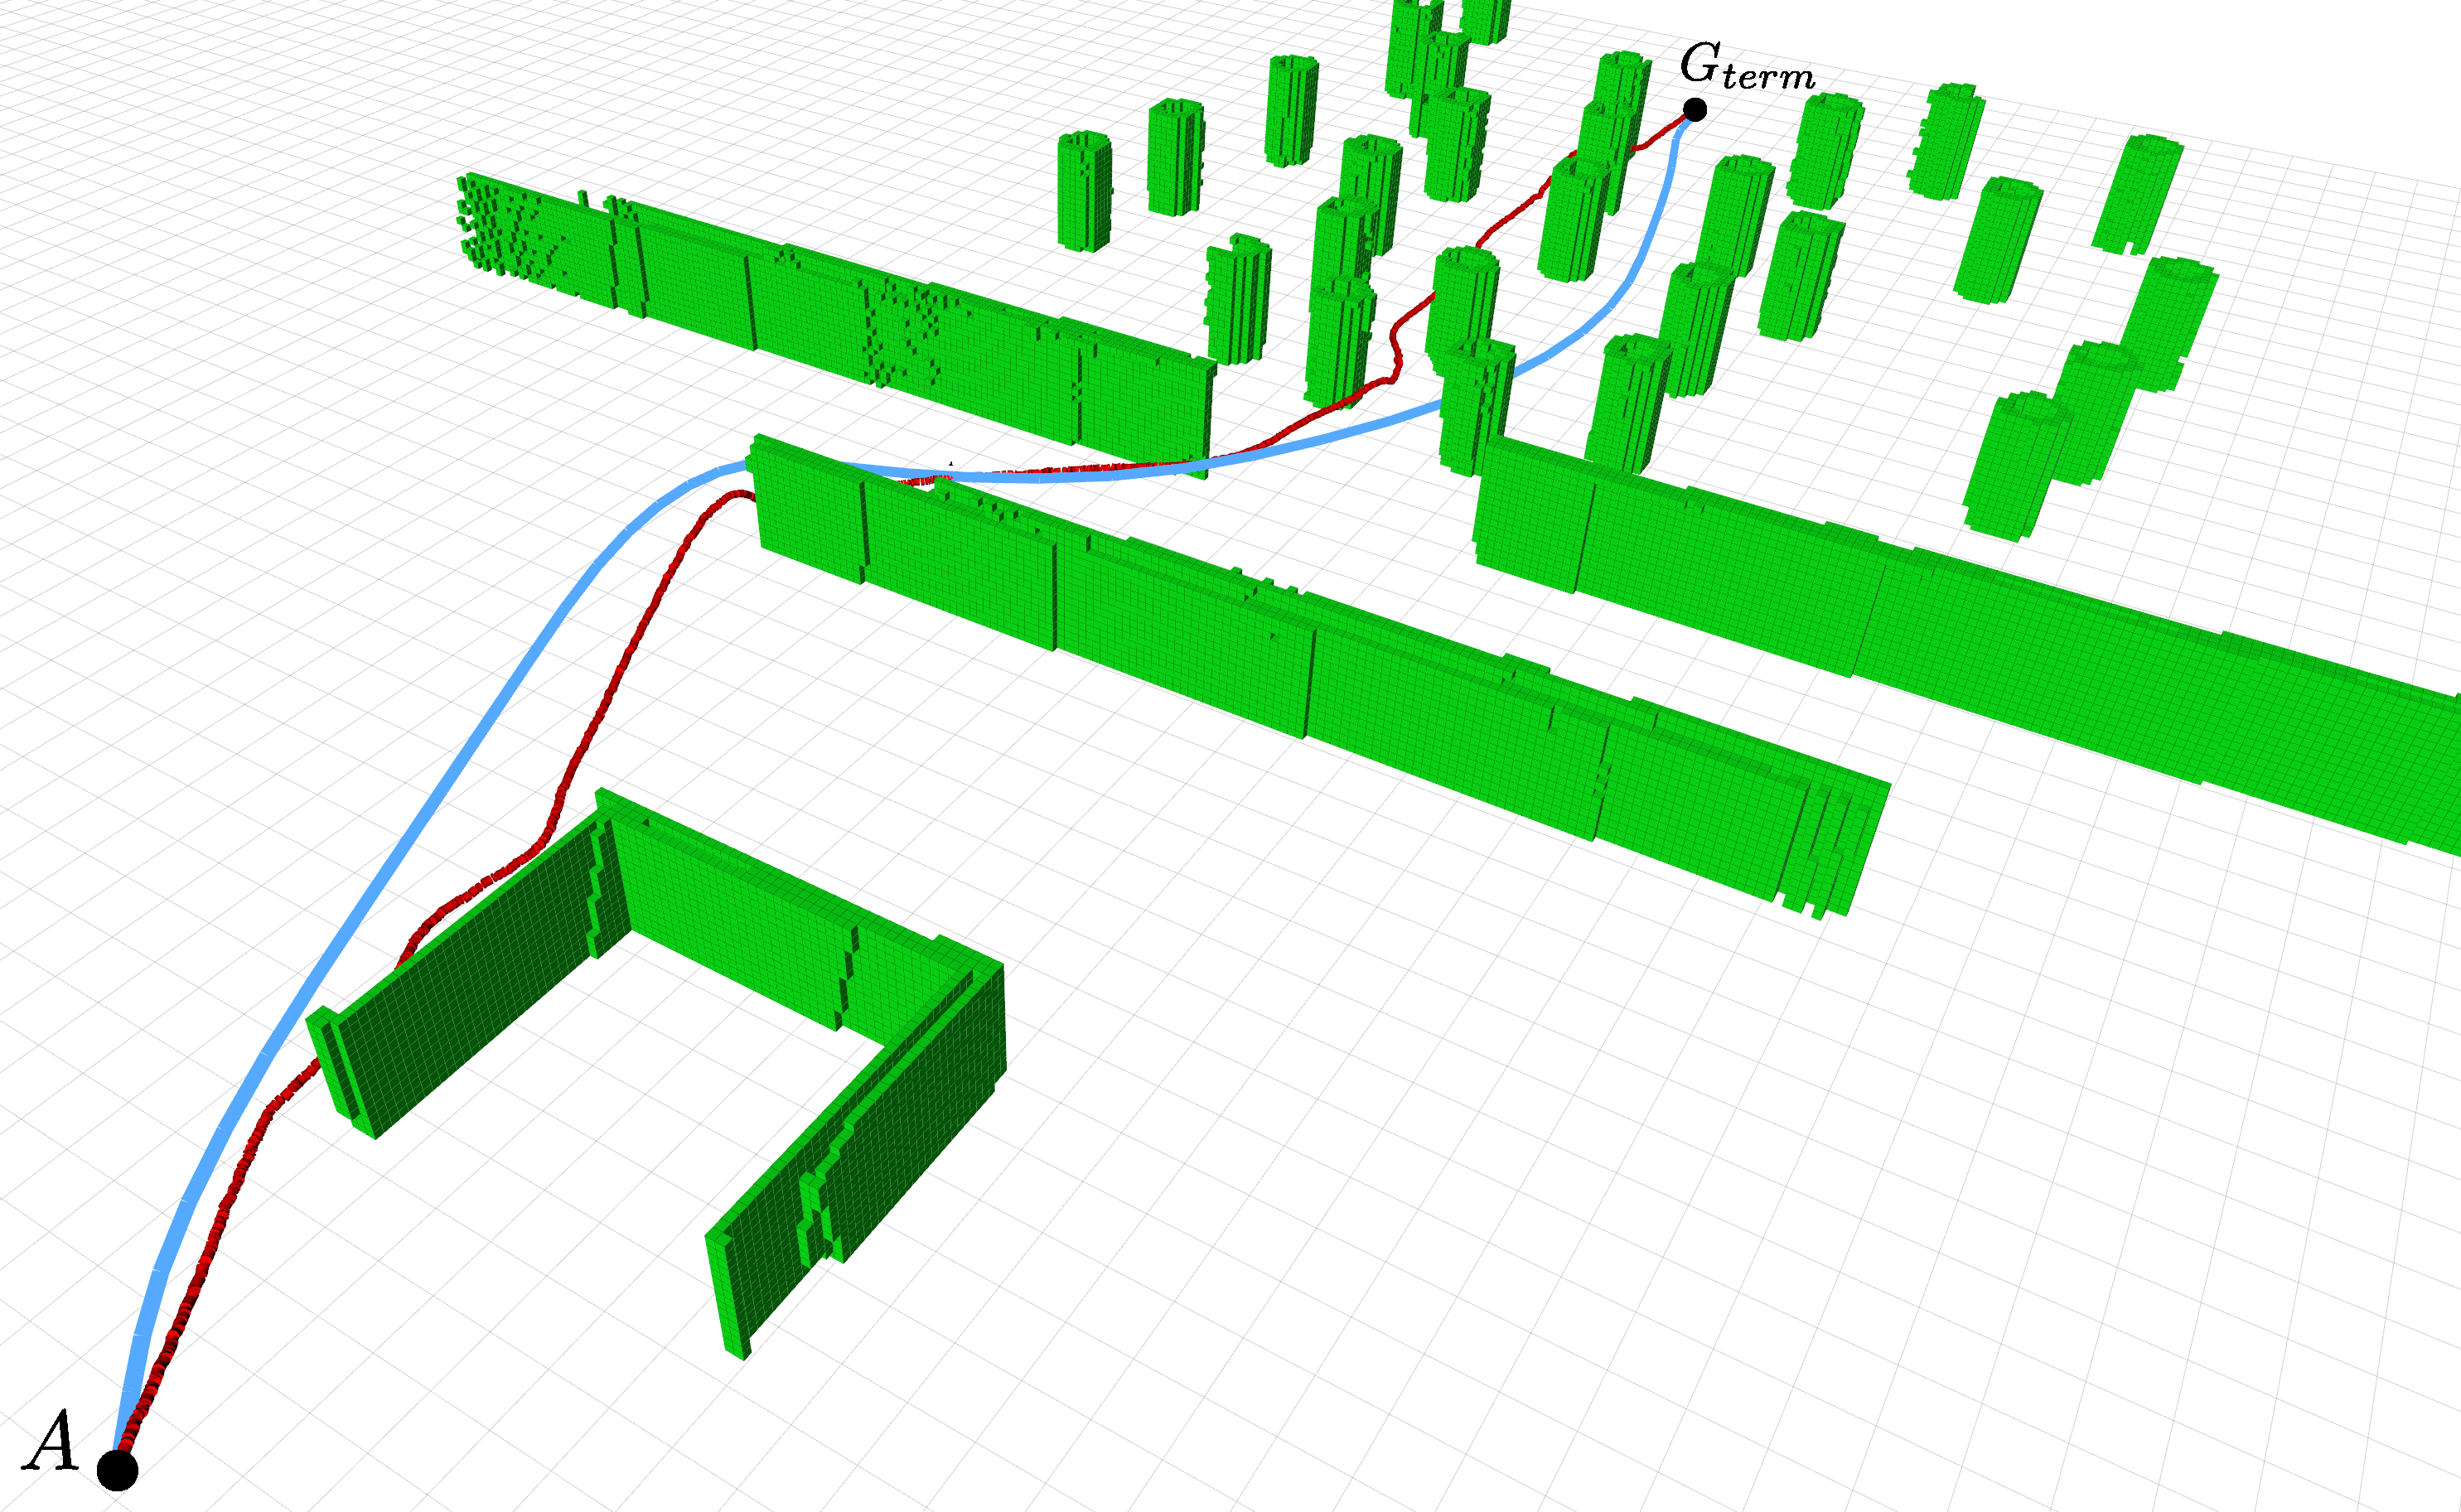
\includegraphics[width=\textwidth]{obstacle_avoidance}$^\dag$\\
      \rule{0in}{1.2em}$^\dag$\scriptsize \url{https://acl.mit.edu/projects/real-time-planning-obstacle-avoidance-uavs}
    }
    \only<5>{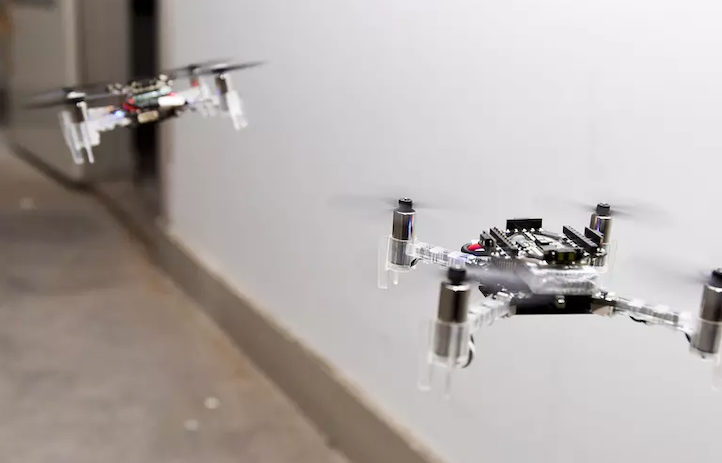
\includegraphics[width=\textwidth]{drone_action}$^\dag$\\
      \rule{0in}{1.2em}$^\dag$\scriptsize Crazyflie drone \url{https://www.bitcraze.io/}
    }
  \end{minipage}
\end{frame}

\section{Antecedentes y motivación para el proyecto}
\begin{frame}{Arquitectura híbrida}
  \begin{minipage}{0.5\textwidth}
    \centering
    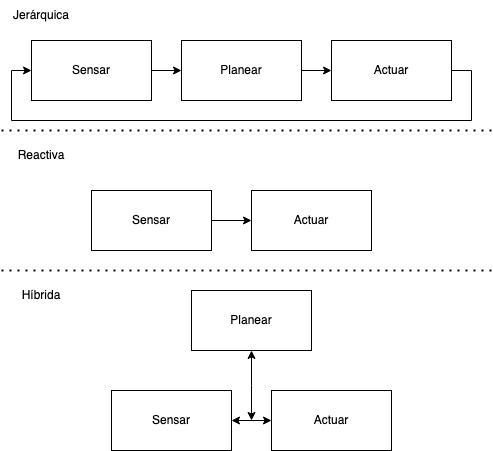
\includegraphics[scale=0.40]{paradigma}$^\dag$\\
    \rule{0in}{1.2em}$^\dag$\scriptsize Paradigmas de arquitectura \url{https://cs.brown.edu/people/tdean/courses/cs148/02/architectures.html}\\
  \end{minipage}
  \begin{minipage}{0.4\textwidth}
    \centering
    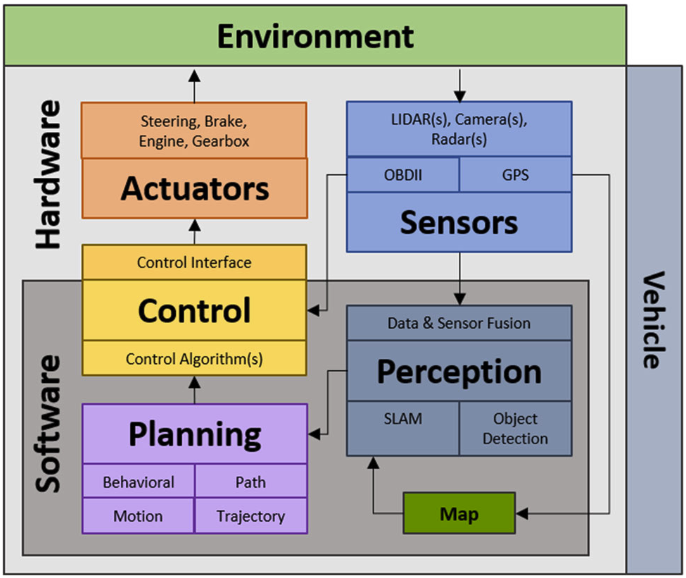
\includegraphics[scale=0.30]{control_autonomo2}$^\ddagger$\\
    \rule{0in}{1.2em}$^\ddagger$\scriptsize Propuesta de una arquitectura de automóvil autónoma \cite{CurielRamirez2019}\\
  \end{minipage}
\end{frame}

\begin{frame}{Multi-robots}
  \begin{columns}
    \column{0.5\textwidth}
    \scriptsize Conjunto de robots que pueden cooperar y comunicarse entre sí para realizar ciertas tareas.\\
    \bigskip % Vertical whitespace
    \scriptsize Ventajas
    \begin{itemize}
      %\item Eficiencia y cobertura
      \scriptsize \item Redundancia y tolerancia a fallos
      %\item Adaptabilidad a entornos dinámicos
      \scriptsize \item Distribución de carga de trabajo
      \scriptsize \item Esfuerzo colaborativo
    \end{itemize}
    \bigskip % Vertical whitespace
    Desventajas
    \begin{itemize}
    \item Complejidad computacional
    \item Comunicación
    \item Mantenimiento
    \end{itemize}
    \column{0.5\textwidth}
    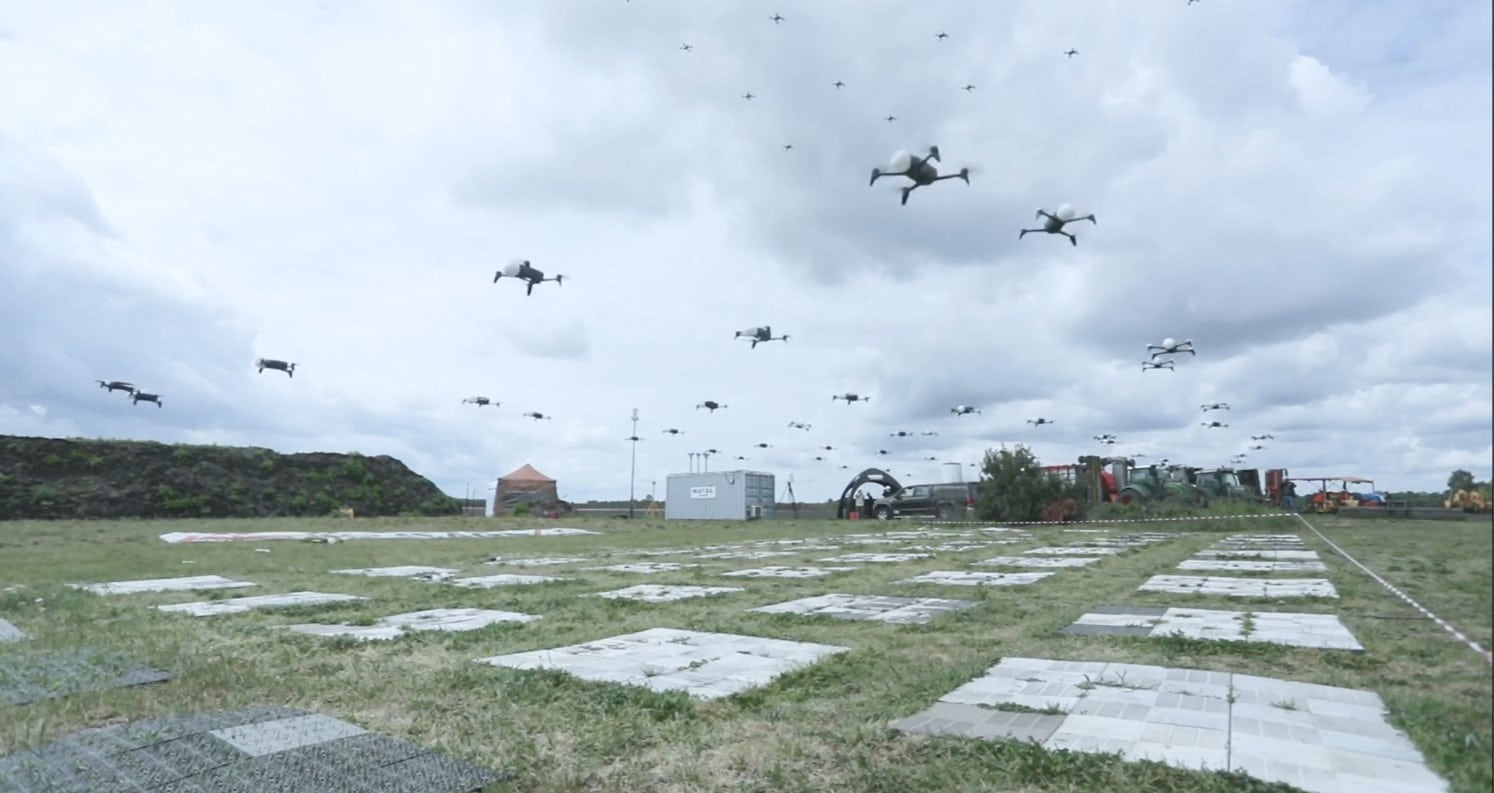
\includegraphics[width=\textwidth]{drone_swarm}$^\dag$\\
    \rule{0in}{1.2em}$^\dag$\scriptsize Enjambre de drones\\ \url{https://www.navalnews.com/naval-news/2022/03/naval-group-teaming-with-french-startup-to-develop-drone-swarm-solutions/}
  \end{columns}
\end{frame}

\begin{frame}{Panorama Planificación de trayectorias}
  %\cite{nphard}[\citenum{nphard}] \cite{5427034}[\citenum{5427034}]
  %Calcular la ruta más corta entre dos puntos en un ambiente 3D es un problema NP-HARD.
  %La mayoria de planificadores de rutas hacen uso de heuristicas y metaheuristicas para
  %generar el óptimo más cercano \\
  \begin{figure}
    \centering
    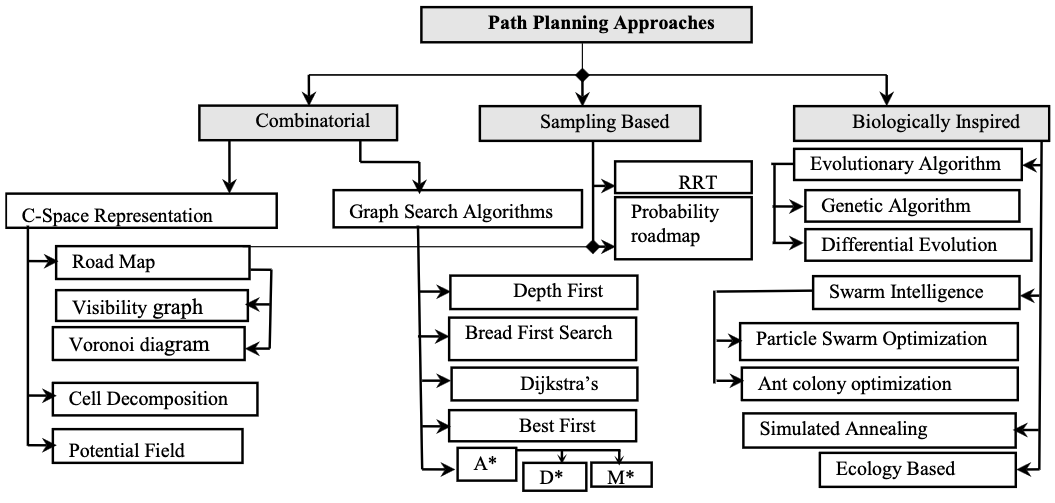
\includegraphics[scale=0.33]{path_planning_panorama}
    \caption[Caption for LOF]{Clasificación del enfoque de planificación de rutas\footnotemark}
  \end{figure}
  \footnotetext{Different Cell Decomposition Path Planning Methods for Unmanned Air Vehicles - A Review \cite{Debnath2020}}
\end{frame}

\begin{frame}{Representación del ambiente 3D}
  %MOSTRAR OCTOMAP
  %MOSTRAR MAPA 3D
  \begin{figure}
    \centering
    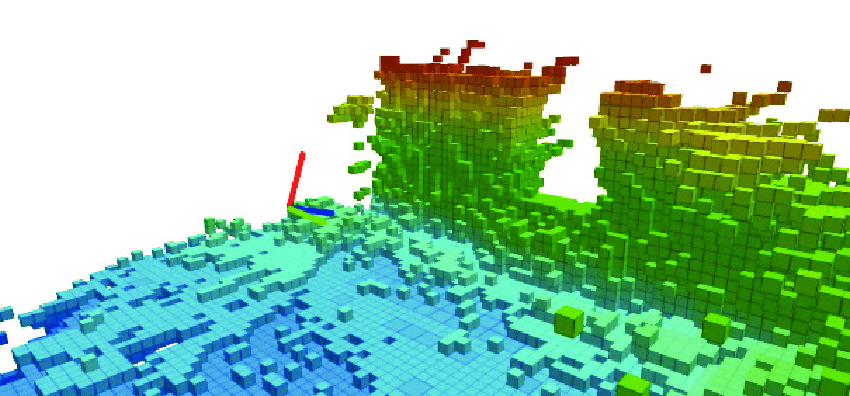
\includegraphics[scale=0.45]{octomapas}$^\dag$\\
    \rule{0in}{1.2em}$^\dag$\scriptsize Mapa probabilistico 3D (Octomap)
    %\caption[Caption for LOF]{Mapa probabilistico 3D\protect\footnotemark}
  \end{figure}
  %\footnotetext{Cooperación en robots heterogeneos}
\end{frame}

\section{Planteamiento del problema}
\begin{frame}
  \frametitle{Planteamiento del problema}
  %\begin{columns}
  %  \column{0.5\textwidth}
  \justifying
  \scriptsize Dada una región tridimensional desconocida y n VANTS, el propósito es encontrar puntos de interés que implique una asignación de trayectoria para cada VANT. En el camino se descubrirán nuevos puntos de interés, haciendo de esta una lista de tareas dinámicas.\\
  El problema consiste en la asignación de tareas de exploración (puntos de visión) para conocer la región de interés, garantizando que toda la región sea explorada, así como la evasión de obstáculos a su paso.\\
  \bigskip % Vertical whitespace
  \pause
  \scriptsize Con base en lo anterior, surgen las siguientes preguntas de investigación:
  \pause
  \begin{itemize}

  \item \scriptsize ¿Cómo se podrá crear una estrategia para optimizar la asignación de tareas y coordinación entre los múltiples VANTS para el problema de exploración de un ambiente desconocido sin señal GPS?
    \pause
  \item \scriptsize ¿Cuál es la representación del medio ambiente de menor complejidad computacional? (para realizar la planificación de trayectorias para los múltiples VANTS)%¿Cómo se pueden diseñar algoritmos rápidos para la planificación de rutas que guie de forma efectiva los múltiples VANTS, considerando la evasión de obstáculos, optimizando la cobertura del área a explorar?
    \pause
  \item \scriptsize ¿Qué mecanismos de coordinación y comunicación pueden facilitar la colaboración y el intercambio rápido de información entre múltiples VANTS durante las misiones de exploración?
    %\pause
  %\item \scriptsize ¿Cómo asegurar que la información que aporte cada uno de los VANTS se integre correctamente a la información ya conocida para generar mapas precisos y completos del entorno explorado?
  \end{itemize}
  
   % \column{0.5\textwidth}\\
   % \pause
   % \centering
   % \small Retos multi-VANT
   % \begin{itemize}
   % \small \item Coordinación% - Establecer comunicación efectiva entre los múltiples VANTs. Intercambiar información relevante. Tener baja latencia en su comunicación.
   % \small \item Planificación% - Los VANTs deben coordinar sus movimientos para evitar colisiones y lograr una cobertura eficiente del área objetivo.
   % \small \item Asignación de tareas% - Se busca evitar la duplicación de esfuerzos optimizando el uso de recursos disponibles.
   % \end{itemize}
   %\end{columns}
\end{frame}

\section{Hipótesis y Objetivos}

\begin{frame}{Hipótesis}

  La implementación de una estrategia de exploración coordinada utilizando múltiples vehículos aéreos no tripulados (multi-VANT) en entornos complejos, permitirá obtener mejores resultados en comparación con la exploración individual (mono-VANT). Esta coordinación eficiente se traducirá en una reducción del tiempo y los recursos necesarios para completar la exploración, así como en una mayor cobertura del área de interés. Además, se espera que la exploración coordinada multi-VANT mejore la calidad de los datos recopilados, lo que permitirá tomar decisiones más informadas y eficaces en diversos campos, como la cartografía, la vigilancia, el monitoreo y la respuesta a desastres naturales.

  
  %La implementación de una arquitectura descentralizada integrada de algoritmos para la detección y evasión de obstáculos, toma de decisiones, navegación e inteligencia colectiva para los múltiples VANTS. Así como un enfoque de fusión de datos que integre la información de los sensores de los múltiples VANTS, mejorará la efectividad y conducirá a mejores resultados de exploración en entornos dinámicos e inciertos, incluida una mayor cobertura del área explorada, una mejor recopilación de datos en comparación con un enfoque de un solo VANT.
  
\end{frame}

\begin{frame}{Objetivos generales y específicos del proyecto}
  %\frametitle
  \begin{enumerate}
  \item<1-> General \\
    \bigskip
    Desarrollar una arquitectura de software descentralizada capaz de resolver los problemas de localización, mapeo, navegación y coordinación multi-VANT en ambientes desconocidos y dinámicos para tareas de exploración en interiores.
    \pause
  \item<2-> Particulares\\
    \bigskip
    \begin{itemize}
    \item Evaluar y comparar diferentes algoritmos de coordinación y planificación de vuelo para la exploración coordinada multi-VANT.
      \pause
    \item Realizar pruebas y simulaciones de la solución propuesta en entornos complejos, analizando métricas como tiempo de exploración, cobertura del área de interés y calidad de los datos recopilados.
      
    \end{itemize}
  \end{enumerate}
\end{frame}

%Explicar con el cronograma
\section{Metodología}
\begin{frame}{Metodología/Cronograma}
  \begin{figure}
    \centering
    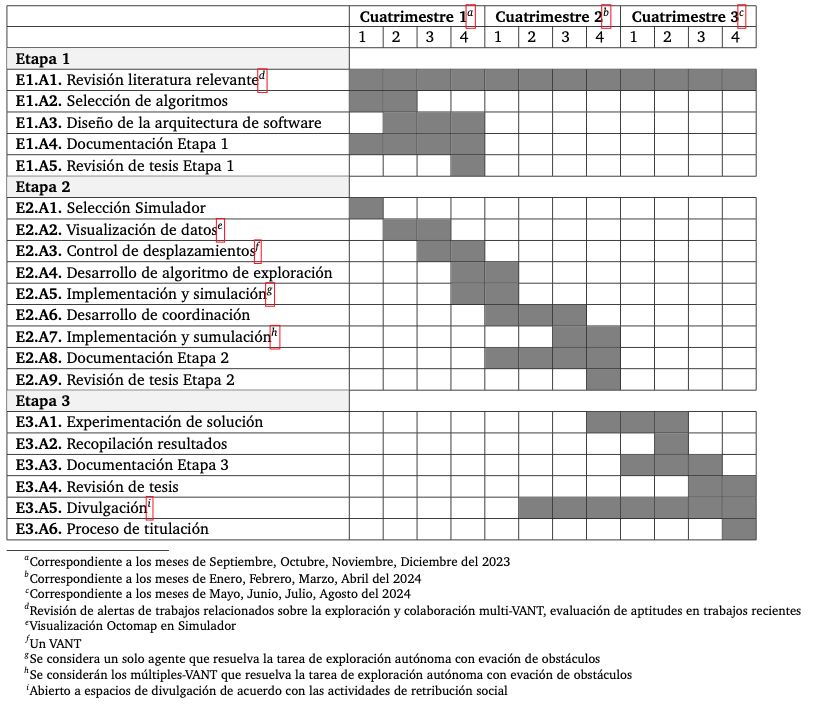
\includegraphics[width=11cm, height=8cm]{cronograma}
  \end{figure}
\end{frame}

\section{Estado del Arte}
\begin{frame}{Estado del Arte}
  \bigskip % Vertical whitespace
  \centering
  \begin{tabular}{ | p{4cm} | p{3cm} | p{2.5cm} | p{3.5cm}|}
    \hline
    \scriptsize REFERENCIA&
    \scriptsize REPRESENTACION&
    \scriptsize BUSQUEDA&
    \scriptsize TRAYECTORIA\\
    \hline
    \hline
    %--------------------------
    \scriptsize \cite{CIESLEWSKI2017}[\citenum{CIESLEWSKI2017}]&
    \scriptsize Octomap&
    \scriptsize Basado en fronteras&
    \scriptsize Control directo de velocidad\\ \hline
    %--------------------------
    \scriptsize \cite{USENKO2017}[\citenum{USENKO2017}]&
    \scriptsize Cuadr\'{i}cula egoc\'{e}ntrica&
    \scriptsize Offline RRT*&
    \scriptsize Curvas de Bezier\\ \hline 
    %--------------------------
    \scriptsize \cite{MOHTA2017}[\citenum{MOHTA2017}]&
    \scriptsize mapa 3D-Local y 2D-Global&
    \scriptsize A*&
    \scriptsize Prograci\'{o}n cuadr\'{a}tica \\ \hline 
    %--------------------------
    \scriptsize \cite{LIN2017}[\citenum{LIN2017}]&
    \scriptsize 3D voxel array TSDF&
    \scriptsize A*&
    \scriptsize Optimizaci\'{o}n cuadr\'{a}tica \\ \hline
    %--------------------------
    \scriptsize \cite{PAPACHRISTOS2017}[\citenum{PAPACHRISTOS2017}]&
    \scriptsize Octomap&
    \scriptsize NBVP&
    \scriptsize Control directo de velocidad \\ \hline
    %--------------------------
    \scriptsize \cite{OLEYNIKOVA2018}[\citenum{OLEYNIKOVA2018}]&
    \scriptsize Voxel Hashing TSDF&
    \scriptsize NBVP&
    \scriptsize Optimizaci\'{o}n cuadr\'{a}tica \\ \hline
    %--------------------------
    \scriptsize \cite{GAO2018}[\citenum{GAO2018}]&
    \scriptsize Mapa de cuadr\'{i}cula&
    \scriptsize M\'{e}todo de marcha r\'{a}pida&
    \scriptsize Optimizaci\'{o}n cuadr\'{a}tica \\ \hline
  \end{tabular}
\end{frame}

\begin{frame}
  
  \centering
  \begin{tabular}{ | p{4cm} | p{3cm} | p{2.5cm} | p{3.5cm}|}
    \hline
    \scriptsize REFERENCIA&
    \scriptsize REPRESENTACION&
    \scriptsize BUSQUEDA&
    \scriptsize TRAYECTORIA\\
    \hline
    \hline
    %--------------------------
    \scriptsize \cite{FLORENCE2018}[\citenum{FLORENCE2018}]&
    \scriptsize Busqueda basada en visibilidad&
    \scriptsize 2D A*&
    \scriptsize Control predictivo por modelo (MPC) \\ \hline
    %--------------------------
    \scriptsize \cite{SELIN2019}[\citenum{SELIN2019}]&
    \scriptsize Octomap&
    \scriptsize Next Best View Planner (NBVP)&
    \scriptsize Control directo de velocidad \\ \hline
    %--------------------------
    \scriptsize \cite{BUG2019}[\citenum{BUG2019}]&
    \scriptsize NA&
    \scriptsize Swarm Gradient Bug Algorithm (SGBA)&
    \scriptsize Control directo de velocidad \\ \hline
    %--------------------------
    \scriptsize \cite{COLLINS2019}[\citenum{COLLINS2019}]&
    \scriptsize KD Tree $+$ Mapa en Voxel&
    \scriptsize B\'{u}squeda en Grafo&
    \scriptsize Movimientos suaves \\ \hline
    %--------------------------
    \scriptsize \cite{CINVES2021}[\citenum{CINVES2021}]&
    \scriptsize Octree&
    \scriptsize Rapidly Exploring Random Trees (RRT)&
    \scriptsize Basado en contornos \\ \hline
    %--------------------------
    \scriptsize \cite{RACER2022}[\citenum{RACER2022}]&
    \scriptsize Octomap HGrid&
    \scriptsize NBVP&
    \scriptsize Control directo de velocidad \\ \hline
    %--------------------------
    \scriptsize \cite{WESTHEIDER2023}[\citenum{WESTHEIDER2023}]&
    \scriptsize Mapa de cuadrícula&
    \scriptsize Deep Reinforcement Learning&
    \scriptsize Control directo de velocidad \\ \hline
    %--------------------------
    \scriptsize \cite{BARTOLOMEI2023}[\citenum{BARTOLOMEI2023}]&
    \scriptsize Mapa de cuadrícula&
    \scriptsize NBVP&
    \scriptsize Control directo de velocidad \\ \hline
    %--------------------------
  \end{tabular}
  
  
  
%\begin{figure}
%  \centering
%  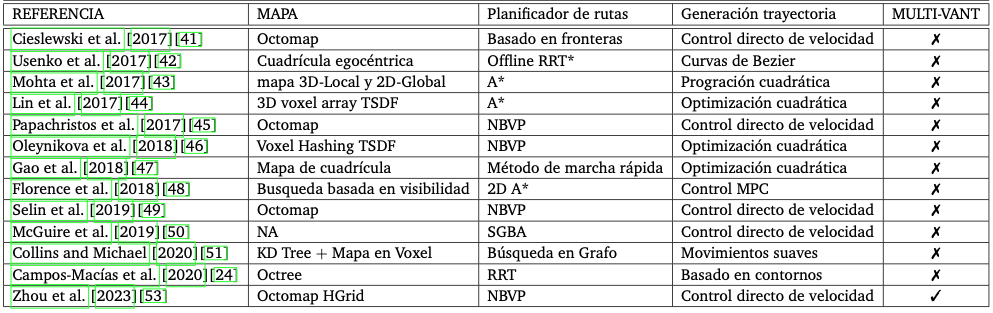
\includegraphics[width=10cm, height=6cm]{estado_del_arte}
%\end{figure}
\end{frame}

\section{Contribuciones o resultados esperados}
\begin{frame}
  \frametitle{Contribuciones o resultados esperados}
  \begin{enumerate}
  \item<1-> Documentación y códigos liberados
    \begin{itemize}
    \item Algoritmo para la exploración multi-VANT
    \item Algoritmo para la planificación de rutas multi-VANT
    \item Protocolo de comunicación y coordinación descentralizados multi-VANT que formaran parte de la arquitectura de software
    \end{itemize}
  \item<2-> Validación de la solución en un simulador
  \item<3-> Tesis impresa
  \end{enumerate}
\end{frame}

\begin{frame}[allowframebreaks,noframenumbering]{Bibliografía}
  \tiny
  \bibliographystyle{abbrvnat}
  \bibliography{test}
\end{frame}

\end{document} 
